\documentclass[10pt,a4paper]{article}
\usepackage[utf8]{inputenc}
\usepackage[T1]{fontenc}
\usepackage[spanish, es-tabla]{babel}

\usepackage{lmodern}
\usepackage{csquotes}

\usepackage{amsmath, amsfonts, amssymb, amsthm}
\usepackage{graphicx}
\usepackage{subcaption}
\usepackage{float}
\usepackage[
    left=2.54cm,
    right=2.54cm,
    top=2.54cm,
    bottom=2.54cm
]{geometry}

\usepackage{tikz}
\usepackage{soul}
\usepackage{listings}

\usepackage[most]{tcolorbox}
\tcbset{shield externalize}

\usetikzlibrary{arrows.meta, positioning, automata}
\usetikzlibrary{babel}
\usetikzlibrary{external}
\tikzexternalize[prefix=build-tikz/]

\usepackage{xcolor}
\usepackage{hyperref}


\lstset{
    language=Python,
    basicstyle=\footnotesize\ttfamily,
    frame=single,
    numbers=left,
    inputencoding=utf8,
    extendedchars=true,
    breaklines=true,
    showstringspaces=false,
    keywordstyle=\color{blue},
    commentstyle=\color{green!50!black},
    stringstyle=\color{red!70!black}
}


\newtcbtheorem[number within=section]{ejercicio}{Ejercicio}{
    enhanced,
    sharp corners,
    boxrule=0pt,
    leftrule=5pt,
    colframe=gray!30!black,
    colback=gray!5!white,
    coltitle=white,
    fonttitle=\bfseries,
    separator sign={.\ },
    before skip=10pt,
    after skip=10pt
}{ej}

\newtcbtheorem[number within=section]{mytheo}{Teorema}{
    enhanced,
    sharp corners,
    boxrule=0pt,
    leftrule=5pt,
    colframe=blue!40!black,
    colback=blue!5!white,
    coltitle=white,
    fonttitle=\bfseries,
    separator sign={.\ },
    before skip=10pt,
    after skip=10pt
}{th}

\newtcolorbox{alerta}[1]{
    enhanced,
    sharp corners,
    boxrule=0pt,
    leftrule=5pt,
    colframe=red!40!black,
    colback=red!5!white,
    coltitle=white,
    fonttitle=\bfseries,
    title=#1,
    before skip=10pt,
    after skip=10pt
}

\newtcolorbox{nota}[1]{
    enhanced,
    sharp corners,
    boxrule=0pt,
    leftrule=5pt,
    colframe=orange!40!black,
    colback=yellow!5!white,
    coltitle=white,
    fonttitle=\bfseries,
    title=#1,
    before skip=10pt,
    after skip=10pt
}


\begin{document}

% PORTADA
\begin{titlepage}

    \centering

    {\huge \textbf{Universidad Nacional Autónoma de México}}\\[0.3cm]

    \rule{\linewidth}{2mm}\\[0.3cm]

    {\large \textbf{Facultad de Estudios Superiores Acatlán}}\\[1cm]

    
\includegraphics[width=6cm]{../../Archivos/Imagenes_Logos/acatlan.png}\\[1cm]

    {\Large \textbf{Matemáticas Aplicadas y Computación}}\\[1cm]

    {\huge \textbf{Database Administrator}}\\[0.5cm]

    \rule{\linewidth}{1mm}\\[0.3cm]

    \vfill

    {\Large \textit{Instalación SGDB}}\\[0.5cm]


    \vfill

    \rule{\linewidth}{0.5mm}\\[0.3cm]

    %{\Large \textit{Ricardo López Ramírez}}\\

    \rule{\linewidth}{0.5mm}\\[0.8cm]

    \small
    Actualización: \today \hfill Página: \thepage

\end{titlepage}


% ÍNDICE
\pagenumbering{roman}

\tableofcontents

\clearpage

\pagenumbering{arabic}

\setcounter{page}{1}

\newpage

\section{Recursos Mínimos del Sistema Operativo}
\vspace{3mm}

Para que MySQL 8 Server pueda ejecutarse, necesita los siguientes recursos.

\begin{itemize}
    \item Procedador \(CPU\): Requiere un procesador con arquitectura de 64bit \(x86\_64\)
    de al menos 1 nucleo.
    \item Memoria \(RAM\): El mínimo para levantar el servicio es 1GB de RAM.
    En la practica para que \(S.O\) y el manejador funcionen sin colapsar, se consideran
    2GB de RAM como minimo.
    \item Disco Duro: Requiere un mínimo de 1GB a 2GB de espacio libre exclusivamente para
    \item instalar el software base \(binario de MySQL\).
\end{itemize}

\subsection{Archivos del S.O (servicios)}

\textbf{Windows} 

Ruta: \texttt{C:\textbackslash Windows\textbackslash System32\textbackslash drivers\textbackslash etc\textbackslash services}
\vspace{3mm}

Al revisar el archivo de servicios del S.O. Windows, se constató que el
puerto de MySQL (3306) no viene registrado por defecto.

Para que el sistema resuelva el nombre del servicio a este puerto a nivel
de red, el administrador debe editar el archivo, agregando manualmente la
siguiente línea al final:

\begin{verbatim}
mysql           3306/tcp               #MySQL Database Server
\end{verbatim}

\begin{figure}[H]
    \centering
    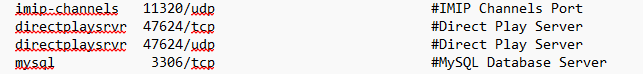
\includegraphics[width=0.8\textwidth]{../Actividad_2/Imagen/tcp.png}
    \caption{SO}
    \label{fig:imagentcp}
\end{figure}


\begin{figure}[H]
    \centering
    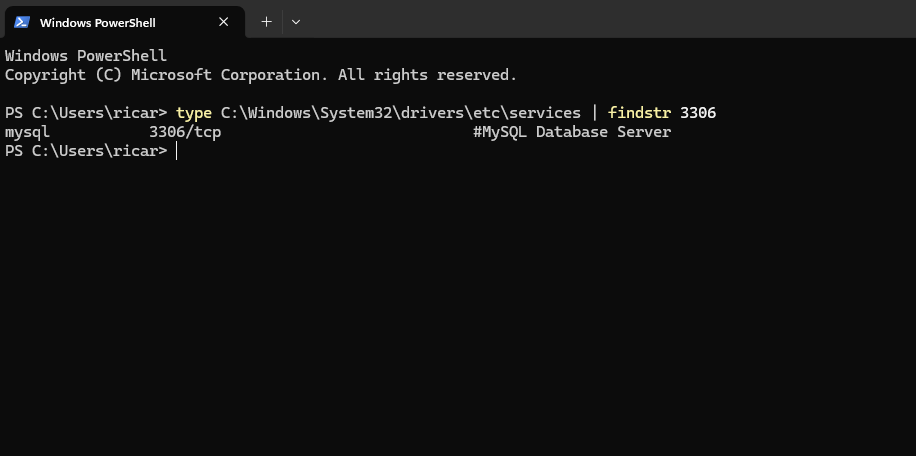
\includegraphics[width=0.8\textwidth]{../Actividad_2/Imagen/tcp3.png}
    \caption{SO}
    \label{fig:imagentcp3}
\end{figure}



\newpage
\subsection{Archivos del S.O (servidores)}

El archivo responsable de mapear las direcciones IP con los nombre de otros servidores
o máquinas de forma local, el archivo hosts.

\vspace{3mm}

\textbf{Windows} 

Ruta: \texttt{C:\textbackslash Windows\textbackslash System32\textbackslash drivers\textbackslash etc\textbackslash hosts}
\vspace{3mm}

\begin{itemize}
    \item El archivo indica que cada entrada debe ir en una línea individual, 
    colocando primero la dirección IP en la primera columna, seguida de al menos un espacio, y luego el nombre del servidor (Host).
    \item El archivo proporciona un ejemplo de cómo mapear un servidor externo.
    \item como se observa al final del archivo, en las versiones modernas de Windows la resolución de localhost (127.0.0.1 o ::1 para IPv6) ya es manejada internamente por el propio DNS del sistema, por lo que estas líneas vienen comentadas por defecto.
\end{itemize}

\begin{figure}[H]
    \centering
    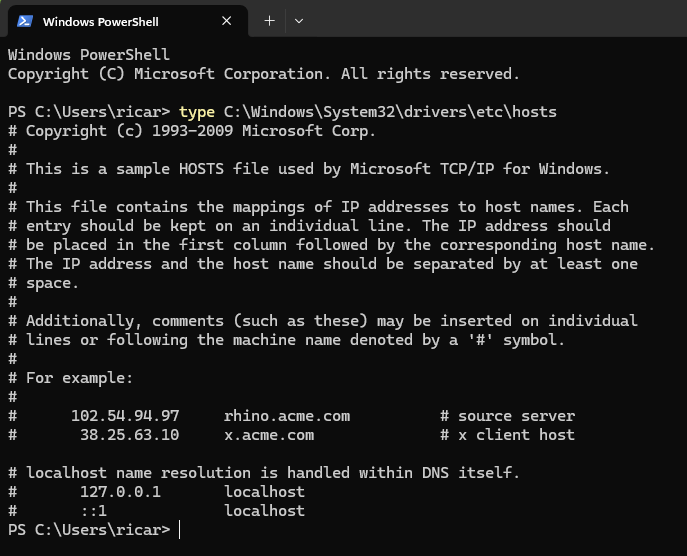
\includegraphics[width=0.8\textwidth]{../Actividad_2/Imagen/tcp2.png}
    \caption{SO}
    \label{fig:imagentcp2}
\end{figure}


\newpage

\section{Instalación MySQL}

\vspace{3mm}

\begin{enumerate}
    \item Ingresamos a la pagina oficial de MySQL: https://www.mysql.com/
    Dirigete al aparatado de DOWNLOADS.
    \item Observa los diferentes productos que puedes seleccionar.
    En este caso se instalara \(MySQL\) Community Edition..
    \item Dependiendo del sistemas operativo, seleccionas la opcion de descarga.
    \item MySQL Installer for Windows
\end{enumerate}


\begin{figure}[H]
    \centering

    \begin{subfigure}{0.48\textwidth}
        \centering
        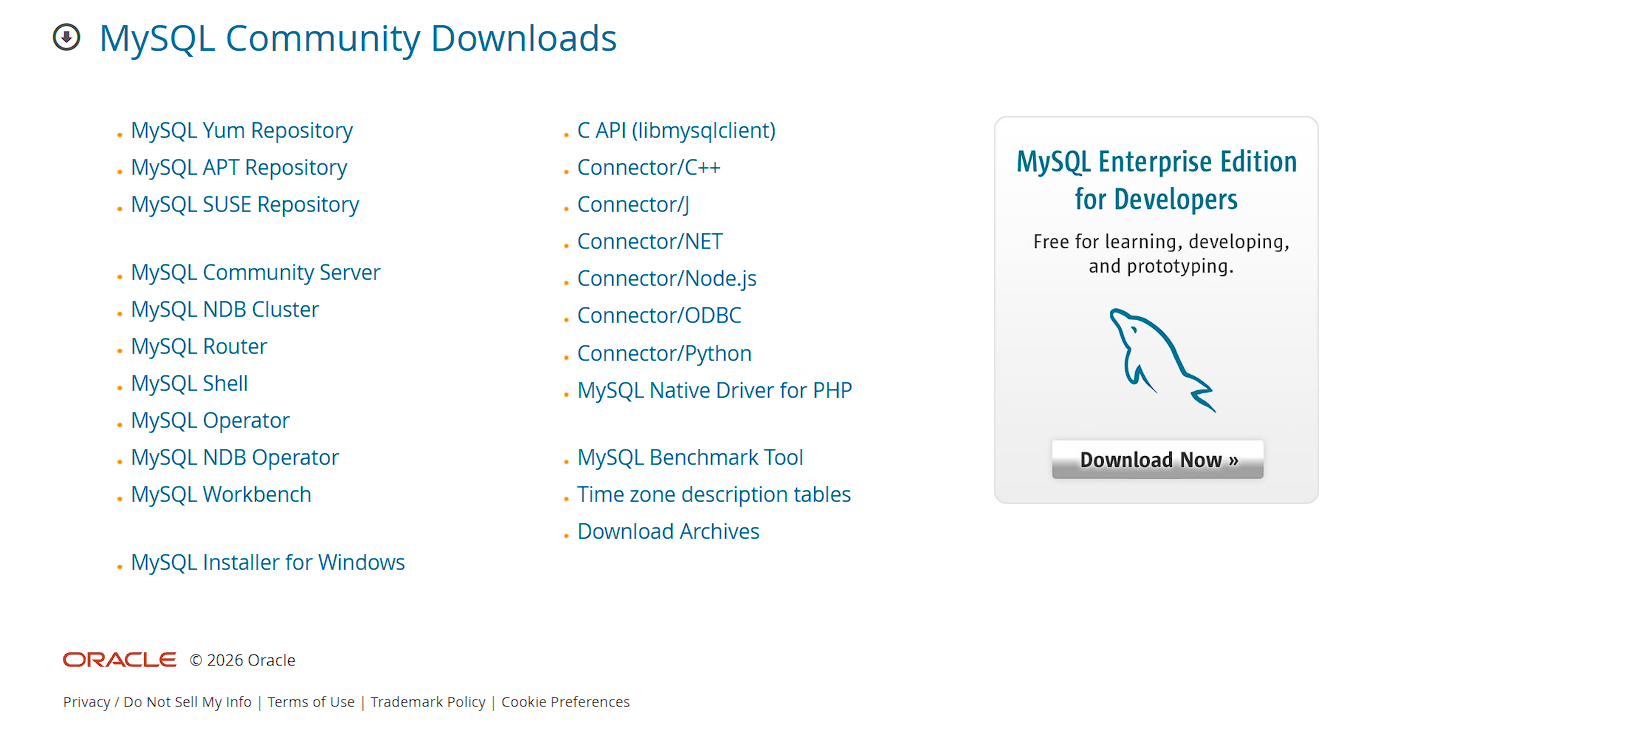
\includegraphics[width=\textwidth]{../Actividad_2/Imagen/Downloads_1.png}
        \caption{Primera etapa de la instalación.}
        \label{fig:instalacion1}
    \end{subfigure}
    \hfill
    \begin{subfigure}{0.48\textwidth}
        \centering
        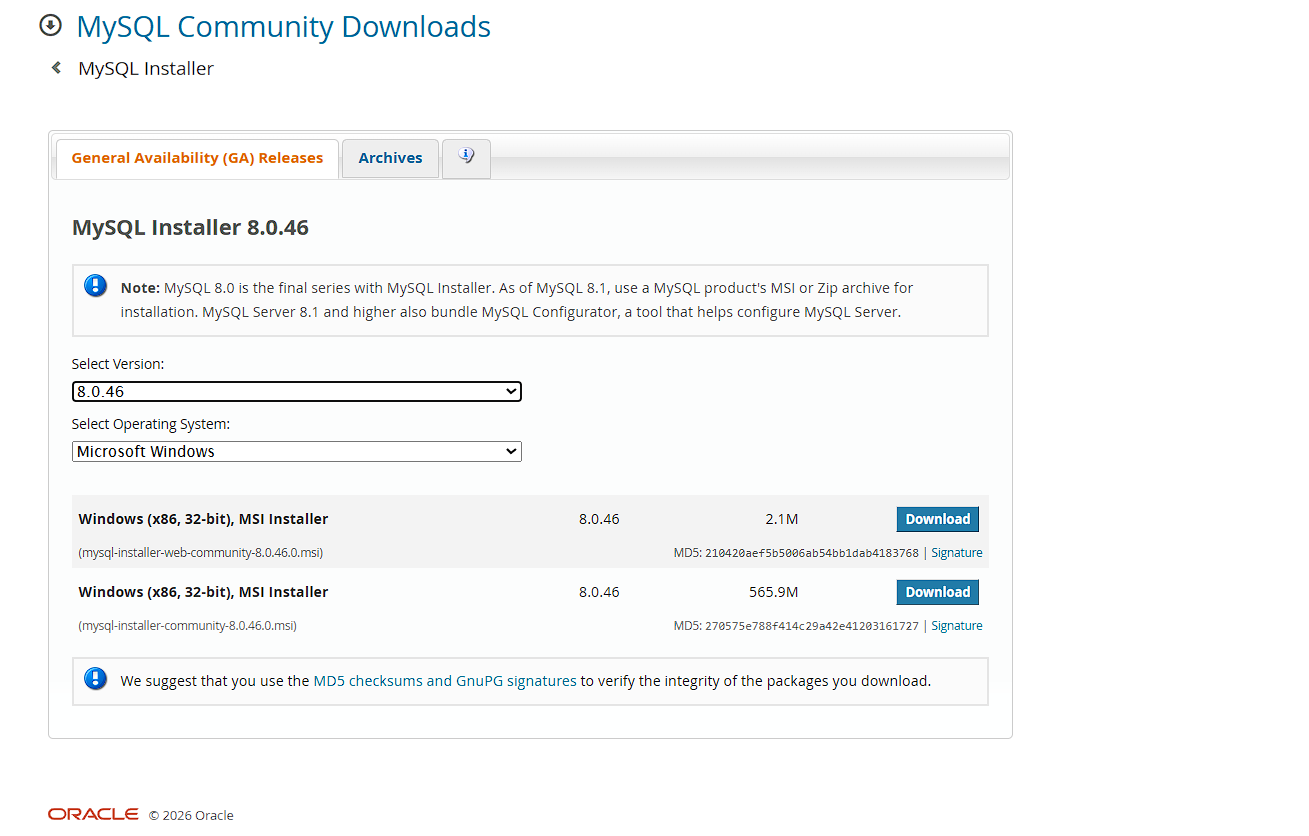
\includegraphics[width=\textwidth]{../Actividad_2/Imagen/Downloads_2.png}
        \caption{Segunda etapa de la instalación.}
        \label{fig:instalacion2}
    \end{subfigure}

    \caption{Proceso de instalación SGDB}
    \label{fig:instalacion_sgbd}
\end{figure}

\vspace{3mm}

Una ves termina la descarga se ejecuta el archivo para iniciar la configuracion SGDB.

\begin{figure}[H]
    \centering
    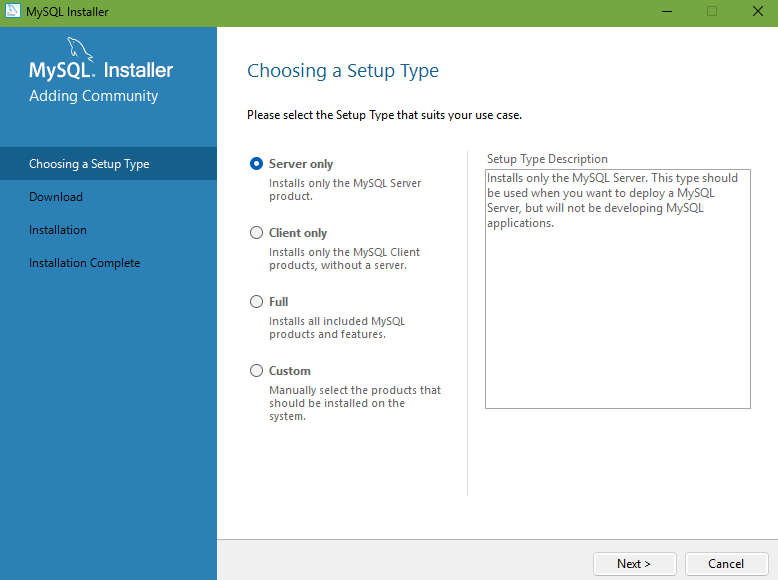
\includegraphics[width=0.8\textwidth]{../Actividad_2/Imagen/Conf_1.png}
    \caption{Ejecucion del programa}
    \label{fig:imagen}
\end{figure}

\newpage
\subsection{Configuracion Inicial del Mysql}

\vspace{3mm}

\begin{itemize}
    \item Tipo de configuración.
    Server Only, Client only, Full, Custom, Dependiendo de las necesidades 
    seleccionas un tipo.
    \item Selecciono Custom, con la siguiente conf.
    \item clicl a Next
    \item Inicia el proceso de descarga e instalacion.
\end{itemize}

\begin{figure}[H]
    \centering

    \begin{subfigure}{0.48\textwidth}
        \centering
        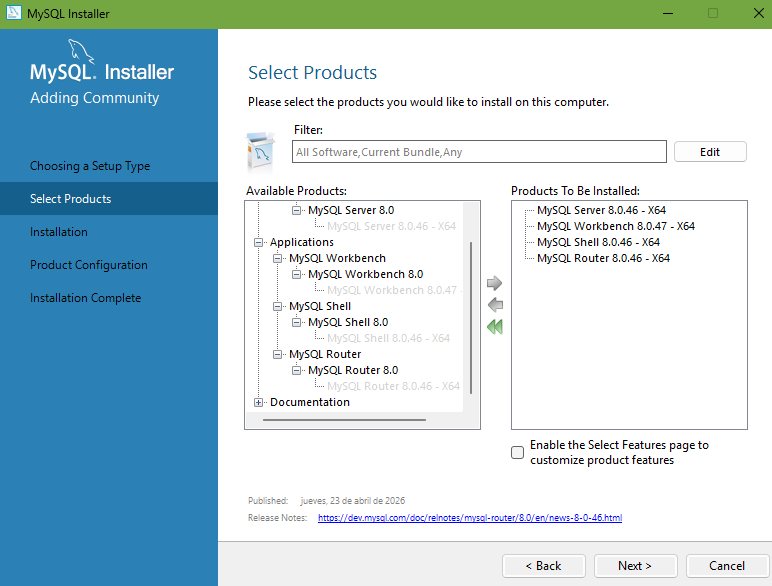
\includegraphics[width=\textwidth]{../Actividad_2/Imagen/Conf_2.png}
        \caption{instalación.}
        \label{fig:instalacion3}
    \end{subfigure}
    \hfill
    \begin{subfigure}{0.48\textwidth}
        \centering
        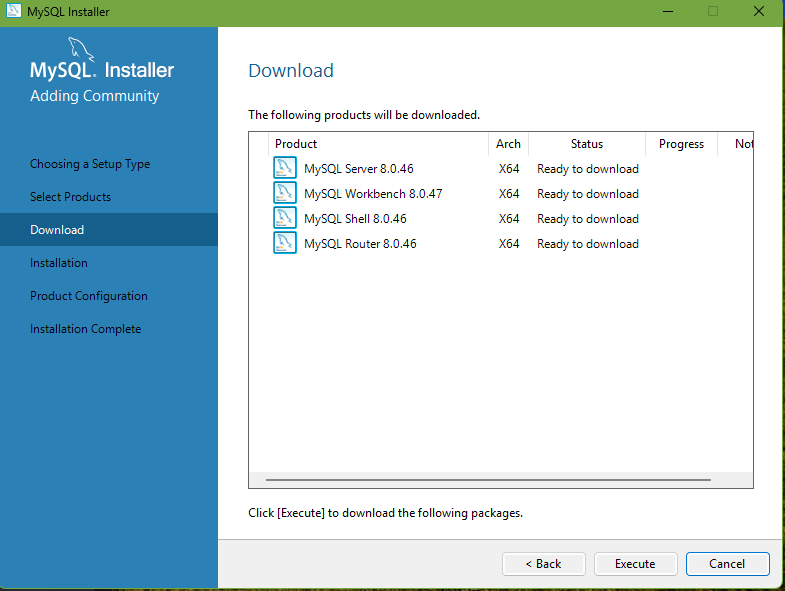
\includegraphics[width=\textwidth]{../Actividad_2/Imagen/Conf_3.png}
        \caption{instalación.}
        \label{fig:instalacion4}
    \end{subfigure}

    \caption{Proceso de instalación SGDB}
    \label{fig:instalacion_sgbd1}
\end{figure}

\vspace{3mm}

\subsection{Tipo de configuración del servidor}

\begin{itemize}
    \item Development Computer.
    \item Server Computer.
    \item Dedicated Computer.
    \item Manual.
\end{itemize}

Para fines de esta instalacion seleccionare Development Computer.
En este aparatdo tambien puede modificar el purto donde escucha MySQL o protocolo.

\begin{figure}[H]
    \centering

    \begin{subfigure}{0.48\textwidth}
        \centering
        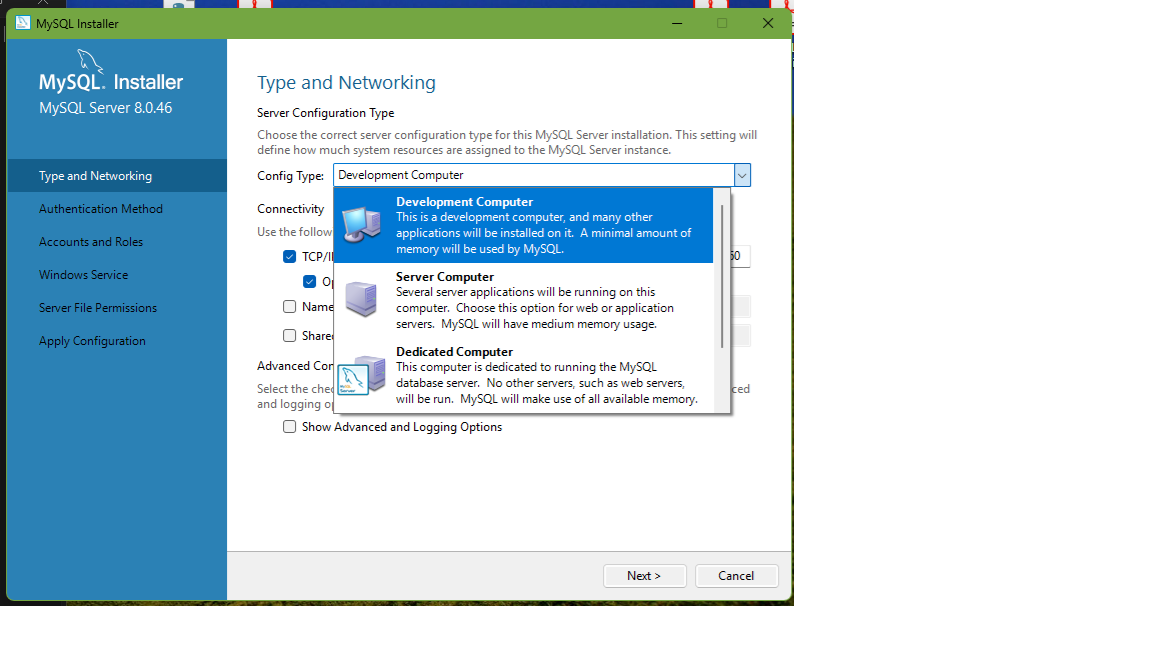
\includegraphics[width=\textwidth]{../Actividad_2/Imagen/Conf_4.png}
        \caption{instalación.}
        \label{fig:instalacion5}
    \end{subfigure}
    \hfill
    \begin{subfigure}{0.48\textwidth}
        \centering
        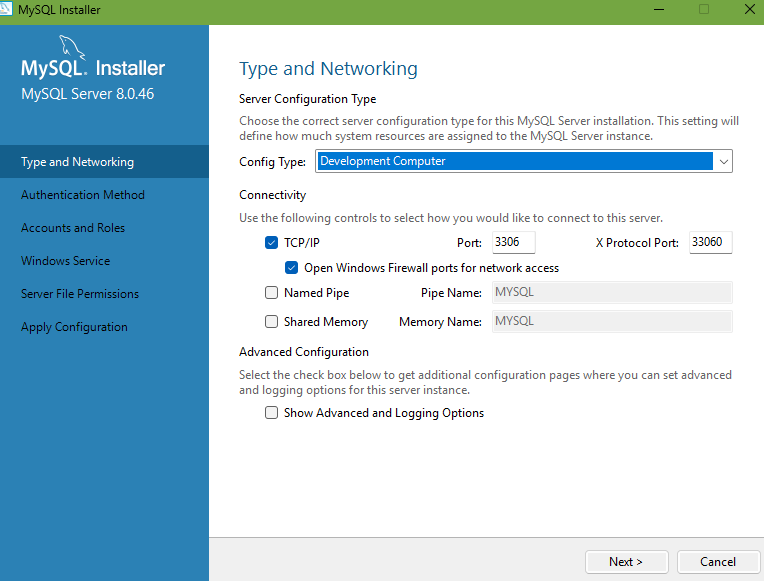
\includegraphics[width=\textwidth]{../Actividad_2/Imagen/Conf_5.png}
        \caption{instalación.}
        \label{fig:instalacion6}
    \end{subfigure}

    \caption{Proceso de instalación SGDB}
    \label{fig:instalacion_sgbd2}
\end{figure}

\vspace{3mm}

\newpage

\subsection{Registro de cuenta y Rol}

\begin{figure}[H]
    \centering
    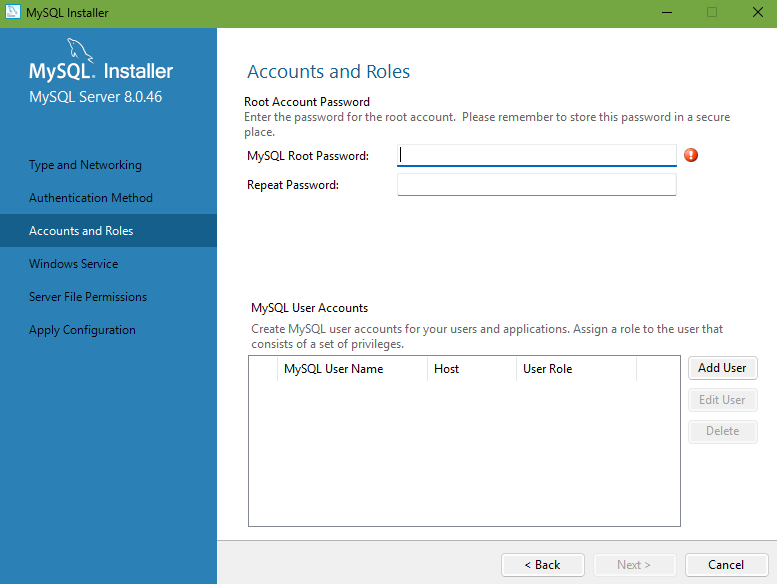
\includegraphics[width=0.8\textwidth]{../Actividad_2/Imagen/Conf_6}
    \caption{Proceso de instalación}
    \label{fig:imagen2}
\end{figure}

Por ultimo se aplica toda la configuracion:

\begin{figure}[H]
    \centering
    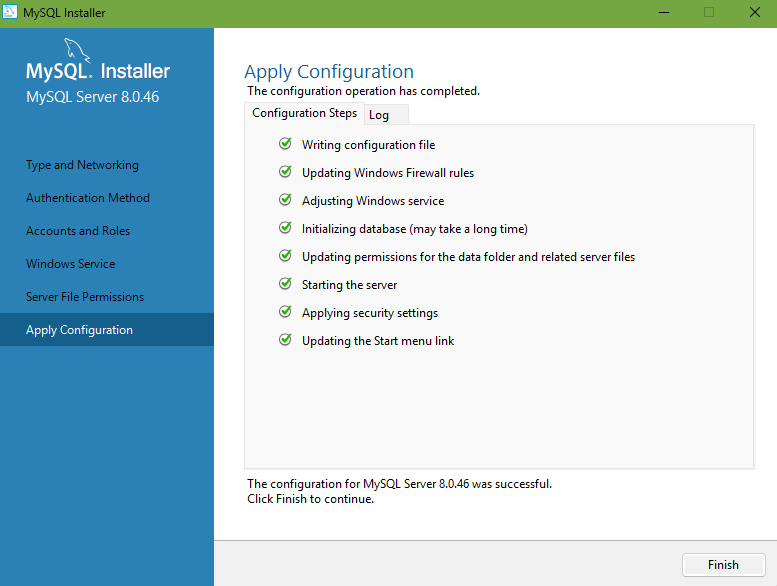
\includegraphics[width=0.8\textwidth]{../Actividad_2/Imagen/Conf_7}
    \caption{Proceso de instalación}
    \label{fig:imagen3}
\end{figure}

\subsection{SGDB en funcionamiento}


\begin{figure}[H]
    \centering
    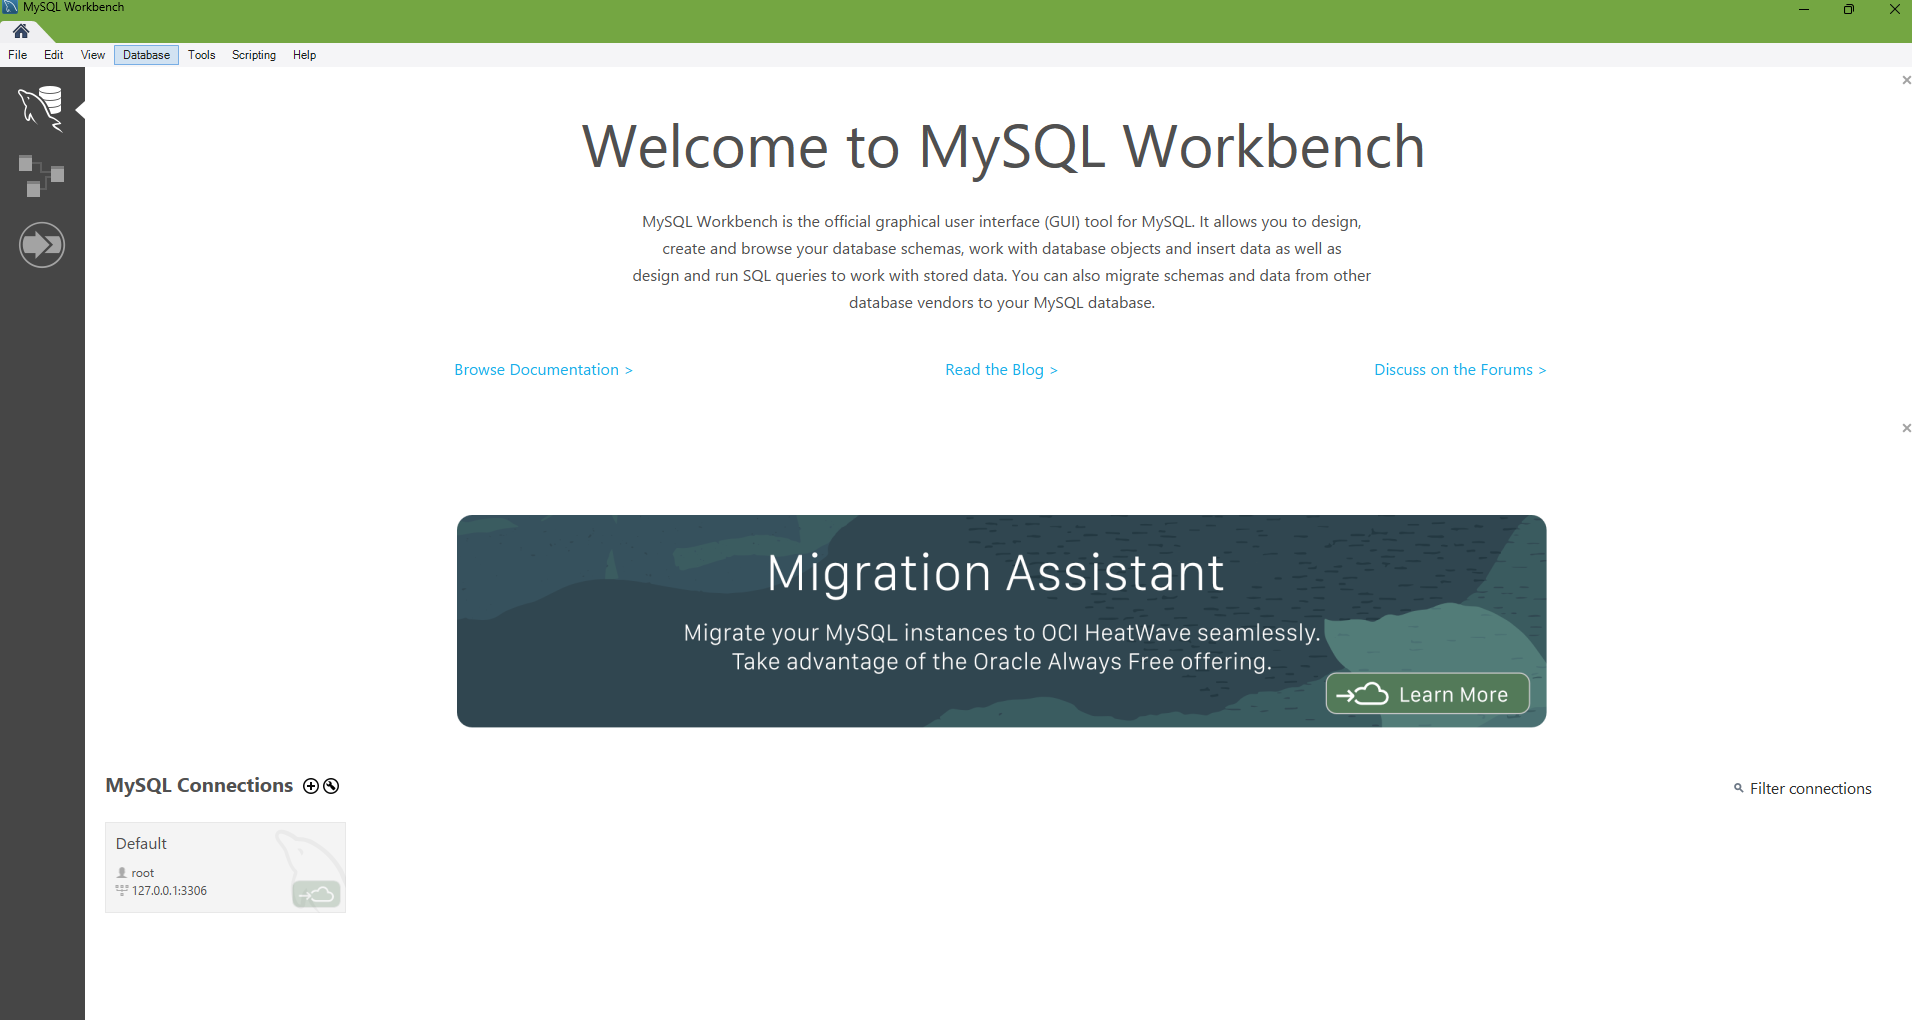
\includegraphics[width=0.8\textwidth]{../Actividad_2/Imagen/Conf_8}
    \caption{Ejecucion del programa}
    \label{fig:imagen4}
\end{figure}

\newpage
\section{Gestión y Control del Servicio}
\subsection{Identificación a nivel S.O.}

\vspace{2mm}

Con el comando \textbf{services.msc} podemos consultar si MySQL está en ejecución.

\begin{itemize}
    \item Detener.
    \item Pausar.
    \item Reiniciar.
\end{itemize}

\vspace{2mm}

\begin{figure}[H]
    \centering
    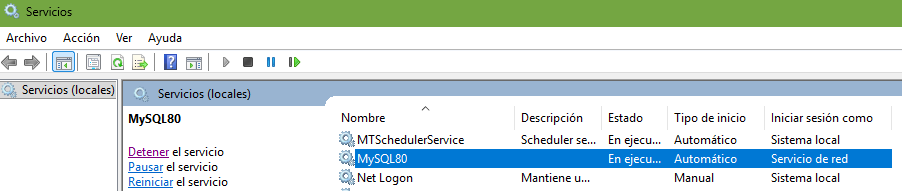
\includegraphics[width=0.8\textwidth]{../Actividad_2/Imagen/ser.png}
    \caption{Servies}
    \label{fig:imagenser}
\end{figure}

\vspace{2mm}

Identificación mediante el controlador de servicios (Comando sc)

\text{sc query MySQL80}

\begin{figure}[H]
    \centering
    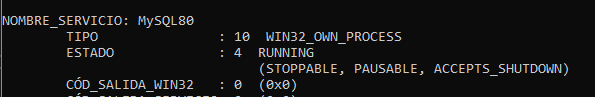
\includegraphics[width=0.8\textwidth]{../Actividad_2/Imagen/sercmd.png}
    \caption{Servies}
    \label{fig:imagensercmd}
\end{figure}

\newpage

\subsection{Control del Servicio}

Servicios(GUI):

Abrir el panel: Presiona las teclas Windows + R, escribe services.msc y presiona Enter.

Levantar y Detener el servicio:

Busca el servicio llamado MySQL80

\begin{figure}[H]
    \centering
    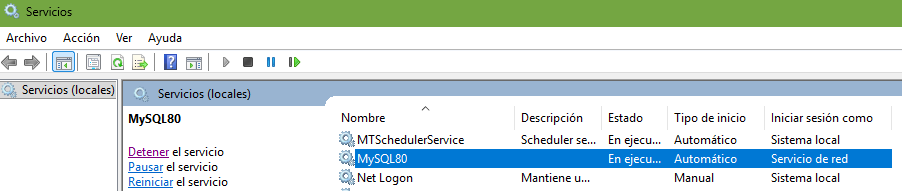
\includegraphics[width=0.8\textwidth]{../Actividad_2/Imagen/ser.png}
    \caption{Servies}
    \label{fig:imagenserr}
\end{figure}

\vspace{3mm}

Comando de S.O.(Consola):
Abre el Símbolo del sistema (CMD) como Administrador. 
Ejecuta los siguientes comandos.

\begin{itemize}
    \item Detener el servicio: net stop MySQL80
    \item Levantar el servicio (Iniciarlo): net start MySQL80
    \item Automatico el servicio: sc config MySQL80 start= auto
\end{itemize}

\begin{figure}[H]
    \centering
    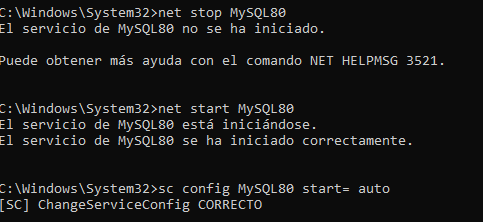
\includegraphics[width=0.8\textwidth]{../Actividad_2/Imagen/servicionet.png}
    \caption{Servies}
    \label{fig:imagensernet}
\end{figure}

\newpage
\section{Referencias}

\begin{thebibliography}{4}

\bibitem{gemini2026}
Google. (2026). \textit{Gemini} (Versi\'on de septiembre) [Modelo de lenguaje grande]. Recuperado de \url{https://gemini.google.com}

\bibitem{iana2024}
Internet Assigned Numbers Authority. (2024). \textit{Service Name and Transport Protocol Port Number Registry}. Recuperado de \url{https://www.iana.org/assignments/service-names-port-numbers/service-names-port-numbers.xhtml}

\bibitem{mysql2024}
Oracle Corporation. (2024). \textit{MySQL 8.0 Reference Manual}. Recuperado de \url{https://dev.mysql.com/doc/refman/8.0/en/}

\bibitem{oracle2024}
Oracle Corporation. (2024). \textit{Oracle Database Documentation}. Recuperado de \url{https://docs.oracle.com/en/database/}

\end{thebibliography}

\end{document}